% Created 2022-12-09 Fri 15:53
% Intended LaTeX compiler: pdflatex
\documentclass[11pt]{article}
\usepackage[utf8]{inputenc}
\usepackage[T1]{fontenc}
\usepackage{graphicx}
\usepackage{longtable}
\usepackage{wrapfig}
\usepackage{rotating}
\usepackage[normalem]{ulem}
\usepackage{amsmath}
\usepackage{amssymb}
\usepackage{capt-of}
\usepackage{hyperref}
\renewcommand\maketitle{}
\usepackage[polish]{babel}
\author{Rafał Grot}
\date{\today}
\title{Wykład 08}
\begin{document}

\maketitle

\section{Sport}
\label{sec:org50f0f58}
\subsection{Stack}
\label{sec:orgf70f6f0}
\begin{verbatim}
#include <iostream>
/*
template <typename T> class IStack {
public:
    virtual void push(const T& data);
    virtual T pop();
    virtual int getCount();
}; */
template <typename T> class Stack // : public IStack<T>
{
    struct Node
    {
        Node* next;
        T data;
    };
    Node* m_fp {nullptr};
    int m_count{};

public:
    void push(const T& data);
    T pop();
    int getCount();
    ~Stack();
    Stack();
};

template <typename T> void Stack<T>::push(const T& data) //O(1)
{
    m_fp = new Node{m_fp, data};
    ++m_count;
}

template <typename T> T Stack<T>::pop() //O(1)
{
    if (m_fp == nullptr)
        return T{};

    T data = m_fp->data;
    Node* toremove{m_fp};
    m_fp = m_fp->next;
    delete toremove;
    --m_count;
    return data;
}

template <typename T> int Stack<T>::getCount() // O(1)
{
    return m_count;
}

template <typename T> Stack<T>::~Stack() //O(N)
{
    while (m_fp != nullptr)
        pop();
}

template <typename T> Stack<T>::Stack() //O(1)
:m_fp{nullptr}, m_count{}
{}

int main()
{
    Stack<int>* stack = new Stack<int>;
    std::cout << stack->getCount() << '\n';  // 0
    stack->push(1); //1
    std::cout << stack->getCount() << '\n'; // 1
    stack->push(2); //21
    stack->push(3); //321
    std::cout << stack->getCount() << '\n'; //3
    std::cout << stack->pop() << '\n'; //21
    std::cout << stack->getCount() << '\n'; //2
    std::cout << stack->pop() << '\n'; //1
    std::cout << stack->pop() << '\n'; //0
    std::cout << "stack empty\n";
    std::cout << stack->pop() << '\n'; // returns default <T> object
}
\end{verbatim}

\begin{verbatim}
0
1
3
3
2
2
1
stack empty
0
\end{verbatim}
\subsection{Queue}
\label{sec:orgaf8ea2c}

\begin{verbatim}
#include <iostream>
/*
template <typename T> class IQueue {
public:
    virtual void enqueue(const T& data);
    virtual T dequeue();
    virtual int getCount();
}; */
template <typename T> class Queue // : public IQueue<T>
{
    struct Node
    {
        Node* next;
        T data;
    };
    Node* m_fp {nullptr};
    Node* m_lp {nullptr};
    int m_count{};

public:
    void enqueue(const T& data);
    T dequeue();
    int getCount();
    ~Queue();
    Queue();
};

template <typename T> void Queue<T>::enqueue(const T& data) //O(1)
{
    Node *newnode = new Node{nullptr, data};
    if(m_fp == nullptr)
        m_fp=newnode;
    if(m_lp != nullptr)
        m_lp->next = newnode;
    m_lp=newnode;
    ++m_count;
}

template <typename T> T Queue<T>::dequeue() //O(1)
{
    if (m_fp == nullptr)
        return T{};

    T data = m_fp->data;
    Node* toremove{m_fp};
    m_fp = m_fp->next;
    delete toremove;
    --m_count;
    return data;
}

template <typename T> int Queue<T>::getCount() // O(1)
{
    return m_count;
}

template <typename T> Queue<T>::~Queue() //O(N)
{
    while (m_fp != nullptr)
        dequeue();
}

template <typename T> Queue<T>::Queue() //O(1)
{}

int main()
{
    Queue<int>* queue = new Queue<int>;
    std::cout << queue->getCount() << '\n';  // 0
    queue->enqueue(1); //1
    std::cout << queue->getCount() << '\n'; // 1
    queue->enqueue(2); //12
    queue->enqueue(3); //123
    std::cout << queue->getCount() << '\n'; //3
    std::cout << queue->dequeue() << '\n'; //23
    std::cout << queue->getCount() << '\n'; //2
    std::cout << queue->dequeue() << '\n'; //3
    std::cout << queue->dequeue() << '\n'; //_
    std::cout << "queue empty\n";
    std::cout << queue->dequeue() << '\n'; // returns default <T> object
}
\end{verbatim}

\begin{verbatim}
0
1
3
1
2
2
3
queue empty
0
\end{verbatim}
\section{Wyklad}
\label{sec:orge655db7}
\subsection{Implementacja Stosu}
\label{sec:orgd67858b}
\begin{verbatim}
class IStack //stack.h
{
public:
    virtual void Put(void* Data)=0;
    virtual void Get(void*& Data)=0;
    __property int Count = {read:GetCout};
    void Free(void);
protected:
    virtual int GetCount(void)=0;
};

class TStack::public IStack //DLL
{
    struct TStackItem
    {
        void* FData;
        TStackItem* FNext;
    };

    TStackItem* FFirst;
    int FCount;
protected:
    void Put(void* AData);
    void Get(void*& AData)
    int GetCount(void)
    void Free(void);
public:
    IStack(void);
    ~IStack(void);
}

IStack* CreateStack(void) //DLL // <- Factory (Export)
{
    return new TStack();
}
//extern "C" IStack __export CreateStack(void);

void TStack::Free(void)
{
    delete this;
}

TStack::TStack(void)
{
    FFirst=NULL;
    FCount=0;
}

TStack::~TStack(void)
{
    void* Data;
    while(FCount) Get(Data);
}

int TStack GetCount(void)
{
    return FCount;
}

void TStack::Put(void* AData)
{
    TStackItem* Item = new TStackItem;
    Item->FData=AData
    Item->FNext=FFirst;
    FFirst=Item
    return ++FCount;
}

void TStack::Get(void*& AData)
{
    TStackItem* Item = FFirst;
    FFirst = Item->Next;
    AData=Item->FData;
    delete Item;
    --FCount;
}

int main(void)
{

    IStack* S = new TStack;
    //IStack* S = CreateStack(); //DLL
    /*
    S->Put(...);
    .;
    .;
    .;
    S->Get(...);
    cout << S->Count; //S->GetCount();
    delete S; // Nie możliwe
    S->Free();
    */
}
\end{verbatim}

$$\text{DLL} \overrightarrow{"Interface, Factory"} \text{APP}$$
\section{Listy dwukierunkowe}
\label{sec:org0e18fe6}
\subsection{Logiczna postać}
\label{sec:orge99c45f}
\begin{description}
\item[{N}] -- next
\item[{P}] -- previous
\item[{F}] -- First
\item[{L}] -- Last
\begin{center}
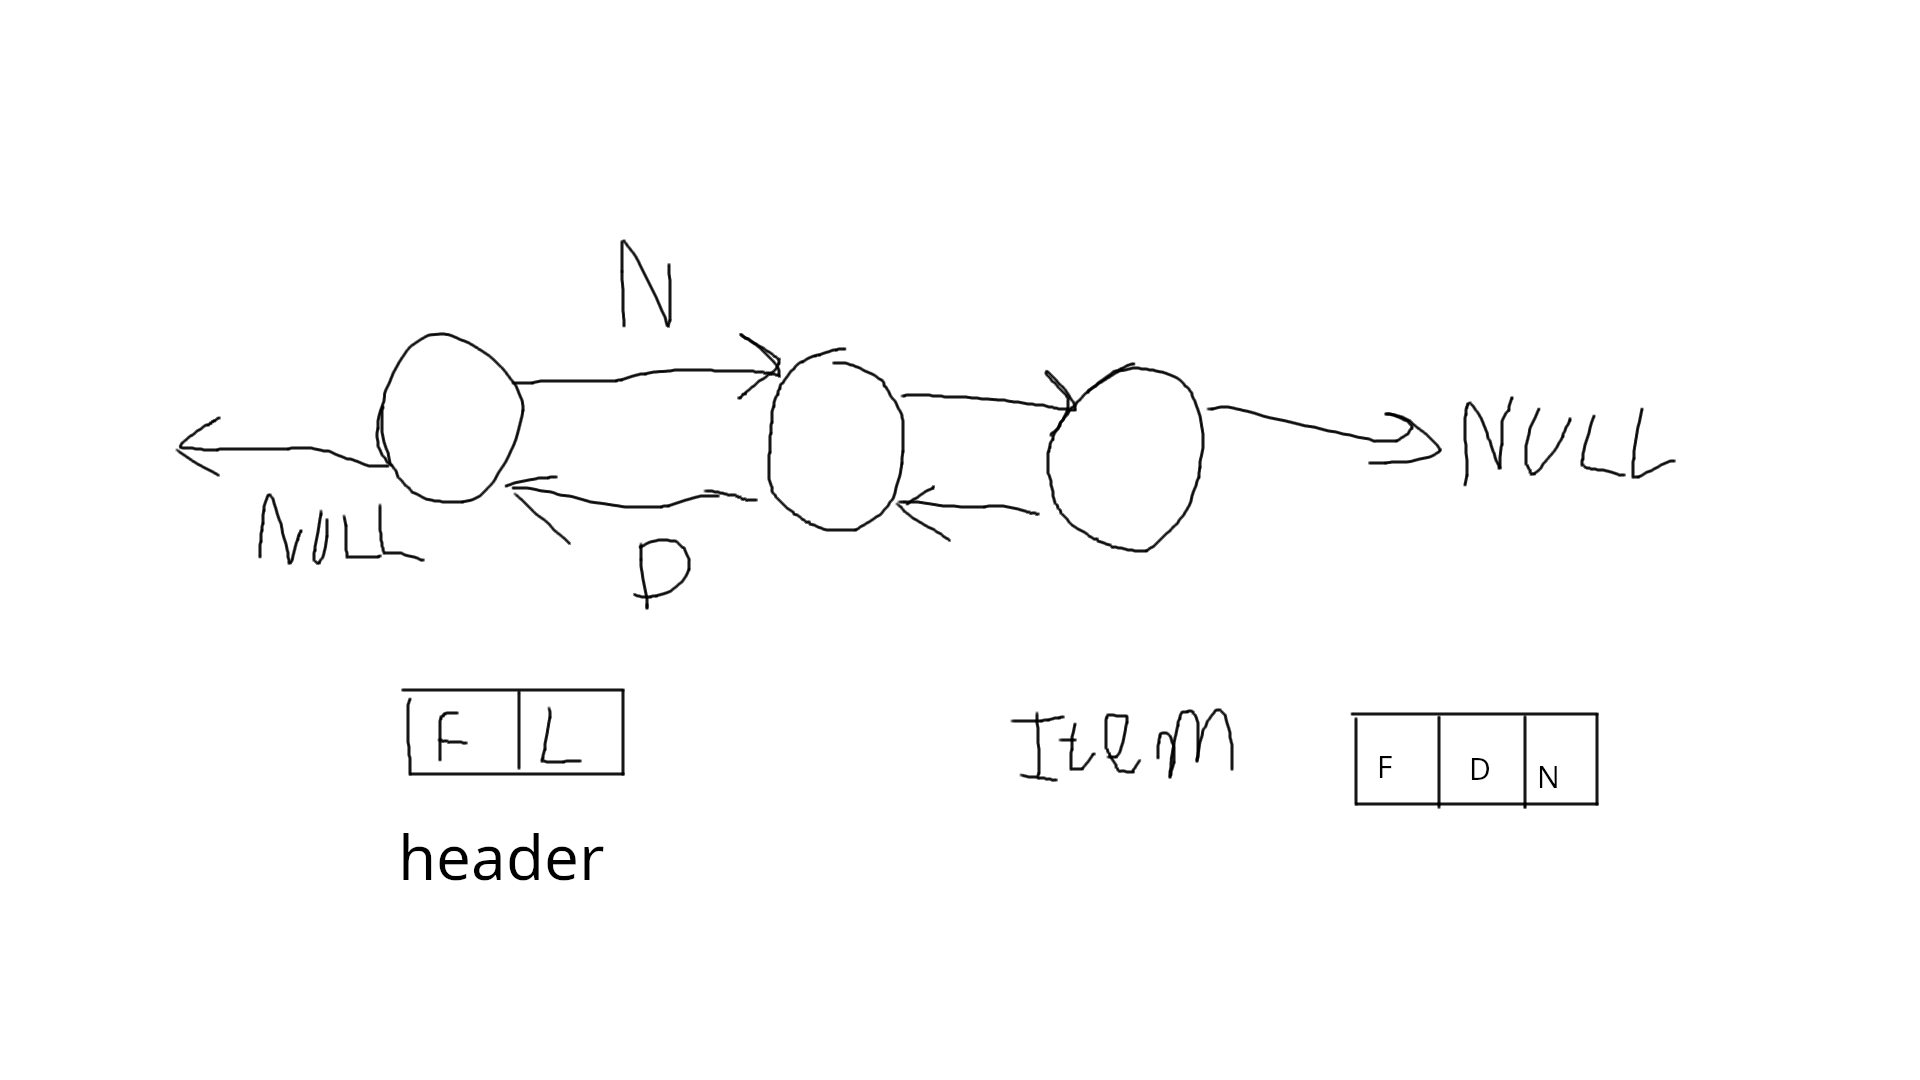
\includegraphics[width=.9\linewidth]{2kierunkowalista.png}
\end{center}
\end{description}
\subsection{Fizyczna}
\label{sec:org9d2b265}
\begin{center}
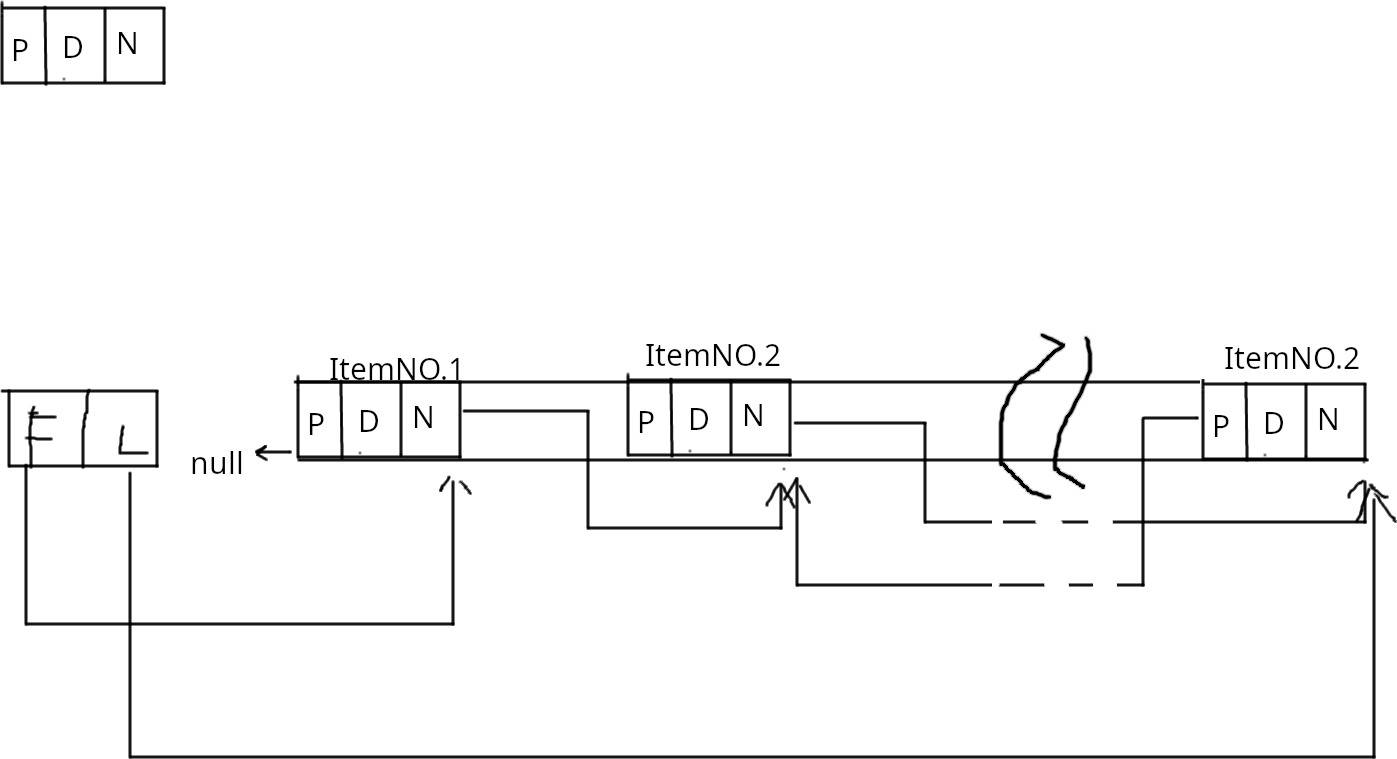
\includegraphics[width=.9\linewidth]{2kierunkowalistafizyczna.png}
\end{center}
\section{Potok}
\label{sec:orgfb9cbc0}
\subsection{1-kier}
\label{sec:org8a2a201}
\begin{itemize}
\item Put
\item Get
\end{itemize}
\subsection{2-kier}
\label{sec:orgf72b046}
\begin{itemize}
\item \texttt{Add}
\item \texttt{Insert(Inode)}
\item \texttt{Delete}
\item \texttt{\_\_propiety Item[Index]};
\end{itemize}
\section{Drzewa binarne}
\label{sec:orgdd43d66}
\subsection{Postać logiczna}
\label{sec:org0deca6a}
\begin{description}
\item[{R}] --root
\item[{L}] --left
\item[{R}] --right
\item[{wyszukwianie}] \(O(\log_{A}N)\)
\end{description}
\section{Drzewa (ogólna postać)}
\label{sec:org9c59ad6}
\section{Grafy}
\label{sec:org5b722c3}
\end{document}